\documentclass[12pt,a4paper]{article}
%per compilare il template usare questo sotto e commentare l'altro:
%\usepackage{../stile}
\usepackage{../../../template/stile}

%Titolo documento
\newcommand{\titoloDocumento}{Template documenti per SWE}

%Prima data di creazione del documento
\newcommand{\dataCreazione}{30 novembre 2015}

%Inserite la versione attuale del documento
\newcommand{\versione}{1.0.0}

%Stato in cui si trova il documento: Formale solo all'atto di consegna
\newcommand{\stato}{Informale || Formale}

%Uso del documento
\newcommand{\uso}{Interno || Esterno}

\rhead{\titoloDocumento}
\lfoot{Versione: \versione}
\title{\titoloDocumento}

\begin{document}
\begin{titlepage}
\begin{center}
\today \\
\vspace{1cm}
\begin{Huge}
\textbf{\nomeTeam}
\end{Huge}
\vspace{1cm}

\includegraphics[scale=0.5]{\logoLungo}
\vspace{1cm}

\HRule \\[0.4cm]
\begin{Huge}
{\huge \bfseries \titoloDocumento}\\[0.4cm]
\end{Huge}
\HRule \\[1cm]
\vfill

\begin{table}[h]
\begin{center}
\begin{tabular}{r | l}
\multicolumn{2}{c}{\textbf{Informazioni sul documento}}\\
\midrule
\textbf{Nome Documento}	&	\titoloDocumento	\\
\textbf{Versione}	&	\versione	\\
\textbf{Stato}	&	\emph{\stato}	\\
\textbf{Uso}	&	\emph{Interno || Esterno}	\\
\textbf{Data Creazione}	&	\dataCreazione	\\
\textbf{Data Ultima Modifica}	&	\today	\\
\textbf{Redazione}	&	Mr X	\\
\ 	&	Mr Y	\\
\ 	&	Mr Z	\\
\textbf{Approvazione}	&	Mr K	\\
\textbf{Verifica}	&	Mr Q	\\
\textbf{Lista distribuzione}	&	\nomeTeam	\\
\ 	&	\Vardanega	\\
\ 	&	\Cardin	\\
\ 	&	Il proponente \Zucchetti	\\

\end{tabular}
\end{center}
\end{table}

\end{center}
\end{titlepage}
\newpage

\Large{\textbf{Registro delle modifiche}}\\
\normalsize

\begin{table}[h]
\begin{center}

\begin{tabular}{p{0.15\textwidth} p{0.3\textwidth} p{0.2\textwidth} p{0.35\textwidth}}
\toprule
\textbf{Versione}	&	\textbf{Autore}	&	\textbf{Data}	&	\textbf{Descrizione}\\
\midrule
\midrule
v1	&	Mr T	&	\today 	&	prima revisione\\
\midrule
v0	&	Mr X	&	30 Febbraio 1959	&	Partenza\\
\bottomrule
\end{tabular}
\caption{Versionamento del documento}
\label{tabVers1}
\end{center}
\end{table}
\newpage

\tableofcontents
\newpage

\listoftables
\listoffigures
\newpage


\section{prova link}
\href{http://docs.oracle.com/javase/tutorial/}{Testo del link}
\newpage

\section{tabella}
\subsection{primo stile}
Testo prima...
\begin{table}[h]
\begin{center}
\rowcolors{2}{light}{}
\begin{tabular}{lcr}
\toprule
titoloC1 - SX	&	titoloC2 - CX	&	titoloC3 - DX\\
\midrule
\midrule
r11	& r12 & r13\\
r21	& r22 & r23\\
r31 & r32 & r33\\
r41 & r42 & r43\\
r51 & r52 & r53\\
\midrule
r61 & r62 & r63\\
\bottomrule
\end{tabular}
\end{center}

\caption{stile colorato}
\label{t1}
\end{table}

Testo dopo...
\newpage

\section{testo con citazioni}
All'uomo solo,\\
ancora pi\`{u} amica,\\
la luna\\
---\\
Yosa Buson
\newpage

\section{codice}
\subsection{C++}
\begin{lstlisting}[basicstyle=\ttfamily]
/*
*	esempio di codice C++
*/
include <iostream>
using namespace std;

main(){
	cout << "Ciao mondo!" <<endl;
}
\end{lstlisting}

\subsection{Java}
\begin{lstlisting}[basicstyle=\ttfamily]
/*
*	esempio di Java
*/
public class Prova{
	public static void main(String[] args){
		System.out.println("Ciao raga ;)");	
	}
}
\end{lstlisting}

\subsection{HTML}
\begin{lstlisting}[basicstyle=\ttfamily]
<!--
Esempio di HTML5
-->
<!DOCTYPE HTML>
<html>
	<body>
	<p>Ciao Web!</p>
	</body>
</html>
\end{lstlisting}
\newpage

%per importare da file:
%\lstinputlisting[language=C++]{main.cpp}

\section{immagine}

\begin{center}
\begin{figure}[h]
\centering
\label{f1-inferno}
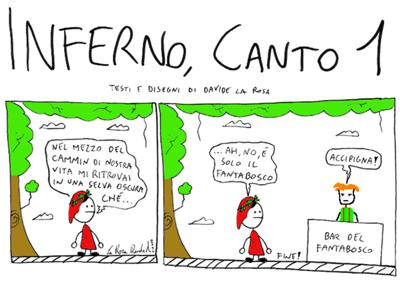
\includegraphics[scale=0.75]{inferno.jpeg}
\caption{Diagramma delle classi dettagliato che illustra i package
\nolinkurl{mytalk.client.iPresenter.iUser.iLogicUser} e mytalk.client.presenter.user.logicUser.}
\end{figure}
\end{center}

Il problema delle \index{immagini} immagini e' che sono difficili da impaginare quando \LaTeX \ f\`{a} i capricci :(
\\
testo a casaccio...\cite{webRTC}
\\
I have been wondering how to make a separate bibliography of my own publications as an appendix in my dissertation. Vincent pointed me to multibib and its siblings, and then I came across this FAQ about all the glories of multiple bibliographies. Doesn’t look like the easiest thing to get going, but I’ll dive into it and see if I manage to get out of it successfully.\cite{som}

%per importare da file:
%\input{sezione.tex}
%\newpage

%per ora non serve la biblio
%\bibliography{../bibliografia}

\end{document}
